\documentclass[11pt,a4paper]{ctexart}
\usepackage{fontspec}
\defaultfontfeatures{Mapping=tex-text}
\usepackage{xunicode}
\usepackage{xltxtra}
%\setmainfont{???}
\usepackage{amsmath}
\usepackage{amsfonts}
\usepackage{amssymb}
\usepackage{graphicx}
\usepackage{amsthm}
\usepackage{array}
\usepackage{float}   %{H}
\usepackage{booktabs}  %\toprule[1.5pt]
\usepackage[titletoc]{appendix}
%===================%插入代码需要的控制
\usepackage{listings}
\usepackage{xcolor}
\setmonofont{Consolas}%字体
\lstset{
	numbers=left, 
	numberstyle= \tiny, 
	keywordstyle= \color{ blue!70},
	commentstyle= \color{red!50!green!50!blue!50}, 
	frame=shadowbox, % 阴影效果
	rulesepcolor= \color{ red!20!green!20!blue!20} ,
	escapeinside=``,% 英文分号中可写入中文
	breaklines=true,
	basicstyle=\ttfamily 
} 
%===================%
\usepackage[left=2cm,right=2cm,top=2cm,bottom=2cm]{geometry}

\newtheorem{theorem}{定理}
\newtheorem{definition}{定义}
\newtheorem*{solution}{解}
\newtheorem{practice}{题}

\title{Time Series HomeWork (10)}
\author{钟瑜 \quad 222018314210044}
\date{\today}
\begin{document}
\maketitle
\pagestyle{plain}%设置页码
\begin{enumerate}
%================================================================%	
	
\item[1.] (q阶)运动平均模型的本质是什么?它有什么特殊性质?它和后面的MA(q)模型有什关系?
\begin{solution}
\begin{enumerate}
	\item[1.]\textbf{ (q阶)运动平均模型的本质:} 有限的线性平稳模型/有限个白噪声的线性组合
	$$ X_t=\sum_{i=0}^{q}b_i\epsilon_{t-i} $$
	
	\item[2.]\textbf{特殊性质:} MA(q) 序列$ \left\lbrace X_t \right\rbrace  $的自协方差函数是q步截尾的;
	\item[3.]\textbf{它和后面的MA(q)模型的关系:}MA(q)模型中的$ b_0=1 $,而(q阶)运动平均模型没有进行约束.
\end{enumerate}
\end{solution}
\item[2.] 如何证明一个时间序列是平稳的? (尽量总结所有方法)
\begin{solution}
\begin{enumerate}
	\item[1.]定义证明:证明二阶矩有限,期望相同且有限,而且自协方差函数只与时间差有关.
	\item[2.]证明$$\sum_{i=0}^{\infty}|a_i|<\infty$$或者$$\sum_{i=0}^{\infty}a_i^2<\infty$$
	\item[3.]证明$ Z_t $为平稳列,其中:
	\begin{figure}[H]
		\centering
		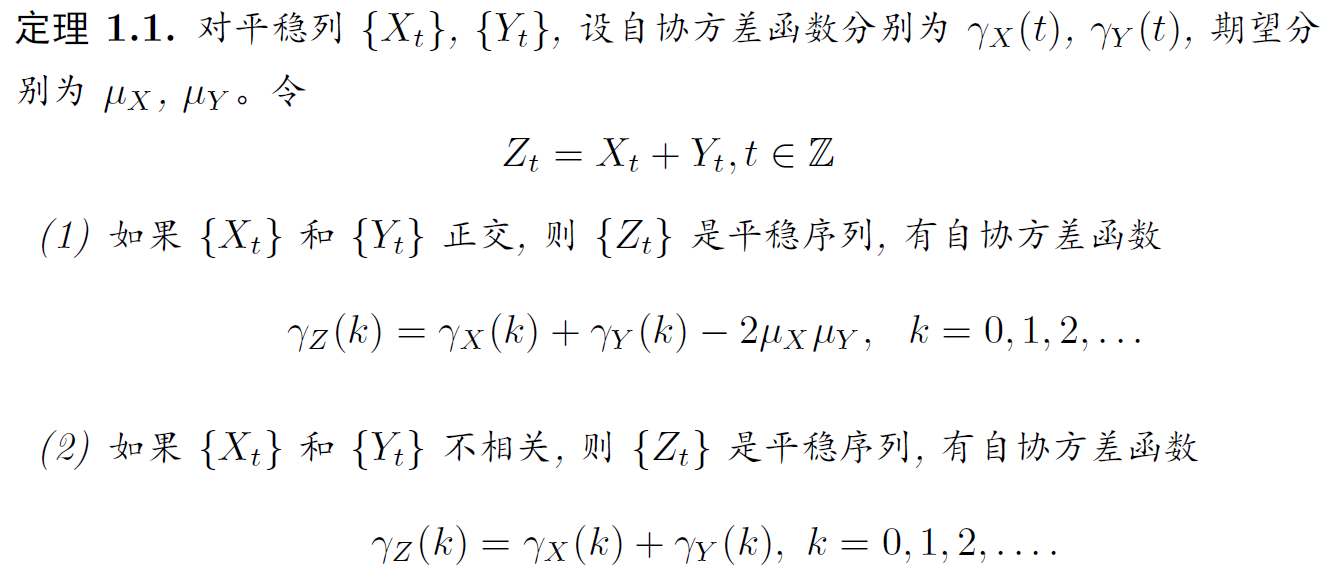
\includegraphics[width=0.75\textwidth]{1.png}  
	\end{figure}
	\item[4.]证明该序列的线性变换之前是一个平稳序列.
	\item[5.]看时序图:平稳就是围绕着一个常数上下波动
\end{enumerate}
\end{solution}

\item[3.] 线性平稳序列和AR模型,MA模型,ARMA模型有什么联系?线性平稳序列的自协方差公式P25(3.5)式在AR模型,MA模型,ARMA模型有什么应用?
\begin{solution}
	1.线性平稳序列和AR模型,MA模型,ARMA模型的联系:
	\begin{figure}[H]
		\centering
		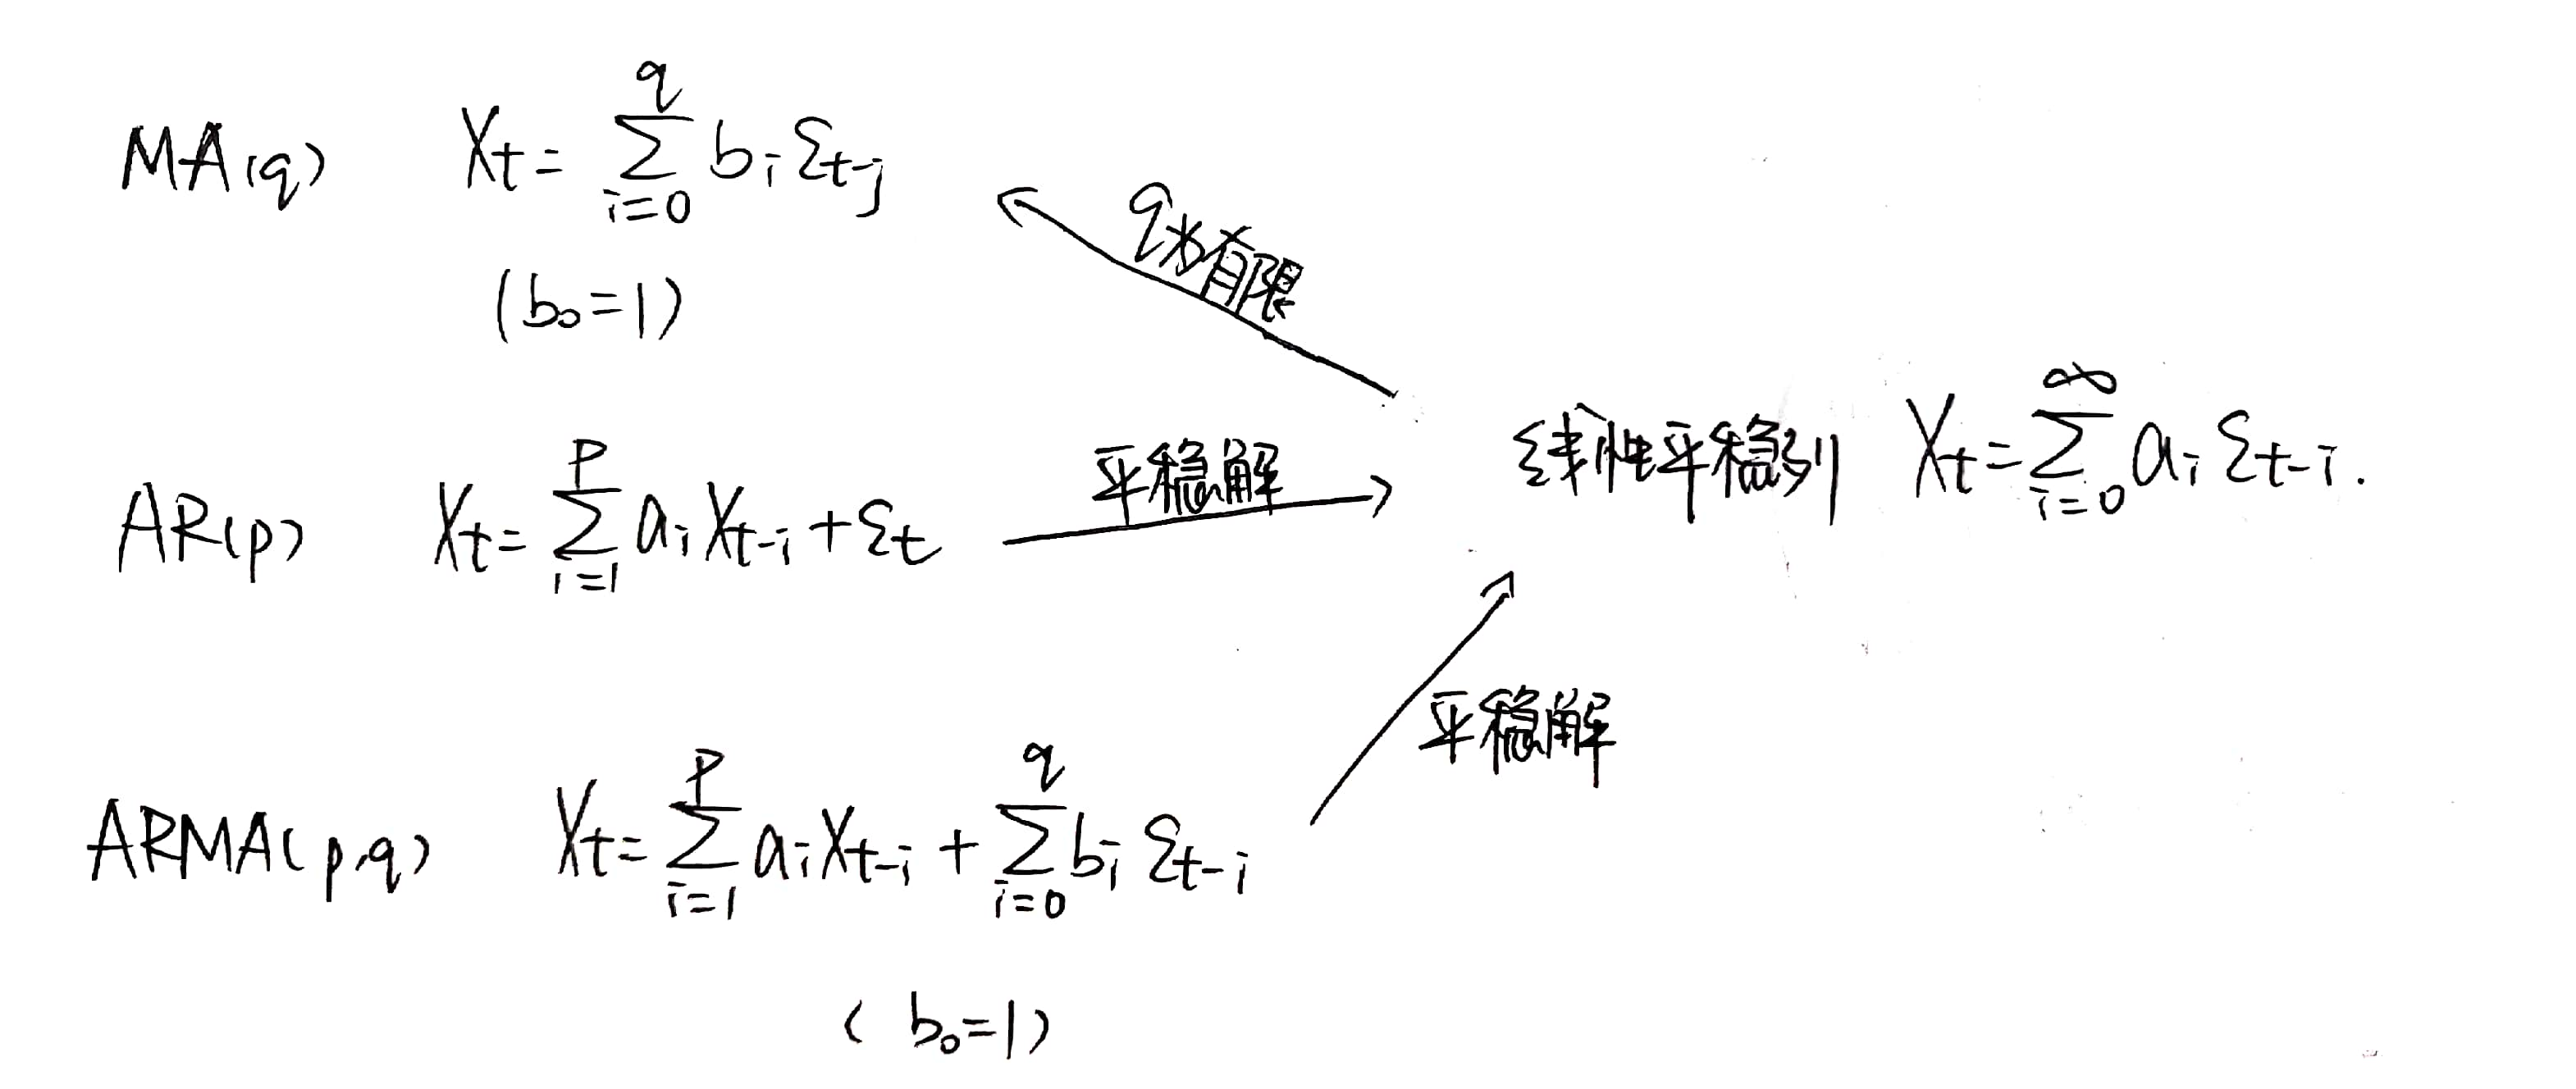
\includegraphics[width=0.75\textwidth]{2.jpg}  
	\end{figure}
2.线性平稳序列的自协方差公式:
\begin{equation}
	\gamma_k=\sigma^2\sum_{j=-\infty}^{+\infty}a_ja_{j+k}
\end{equation}
对于MA(q)模型,$ +\infty $换成$ q-k $
\begin{equation}
	\gamma_k=\sigma^2\sum_{j=0}^{q-k}a_ja_{j+k}
\end{equation}
对于AR(p)模型和ARMA(p,q)模型,a换成$ \psi $
\begin{equation}
	\gamma_k=\sigma^2\sum_{j=-\infty}^{+\infty}\psi_j\psi_{j+k}
\end{equation}

\end{solution}

\item[4.] 严平稳序列和弱平稳序列的关系?你觉得AR(p)序列,MA(q)序列,ARMA(p,q)序列是严平稳的吗?
\begin{solution}
	1.严平稳序列和弱平稳序列的关系:
	\begin{figure}[H]
		\centering
		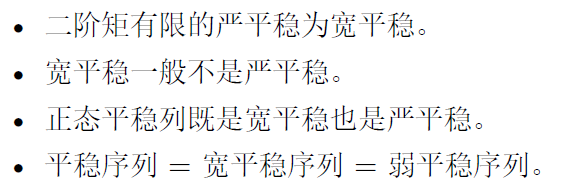
\includegraphics[width=0.4\textwidth]{2.png}  
	\end{figure}

2.不一定.ARMA模型(AR模型和MA模型为ARMA模型的特例)中白噪声项如果是独立同分布的则该平稳列为严平稳遍历。
\end{solution}	

\item[5.]谱密度函数和时间序列的二阶矩有什么关系?P45 线性平稳序列谱密度公式在AR模型,MA模型,ARMA模型中是如何应用的?如何利用谱密度函数来判断时间序列的自协方差函数的周期性?
\begin{solution}
	1. \textbf{谱密度函数和时间序列的二阶矩的关系:}有谱密度的平稳列必为系数平方可和的线性序列,即二阶矩有限.
	
	2. P45 线性平稳序列谱密度公式:
	\begin{figure}[H]
		\centering
		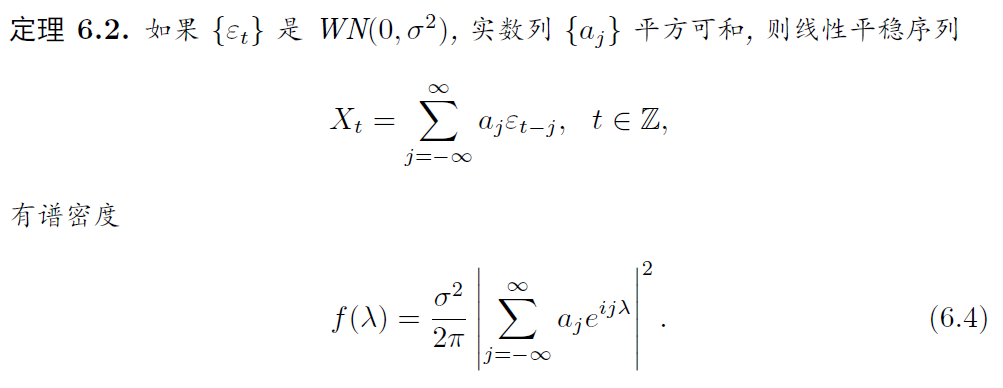
\includegraphics[width=0.75\textwidth]{3.png}  
	\end{figure}
	对于MA(q)模型,由于$$ X_t=\epsilon_t+\sum_{j=1}^{q}b_j\epsilon_{t-j}=B(\mathcal{B})\epsilon_t $$
	故$$f(\lambda)=\frac{\sigma^2}{2\pi}|B(e^{i\lambda})|^2=\frac{1}{2\pi}\sum_{k=-q}^{q}\gamma_ke^{-ik\lambda}$$
	对于AR(P)模型,由于$$X_t=\sum_{i=1}^{p}a_iX_{t-i}+\epsilon_t=A(\mathcal{B})^{-1}\epsilon_t$$
	故$$f(\lambda)=\frac{\sigma^2}{2\pi}|A(e^{i\lambda})^{-1}|^2=\frac{\sigma^2}{2\pi}\frac{1}{|A(e^{i\lambda})|^2}$$
	对于ARMA(p,q)模型,
	\begin{figure}[H]
		\centering
		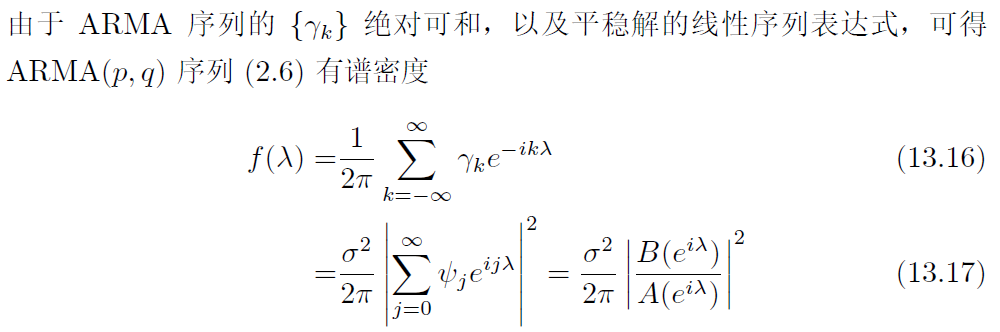
\includegraphics[width=0.70\textwidth]{4.png}  
	\end{figure}
	3.利用谱密度函数来判断时间序列的自协方差函数的周期性:
	
	对于AR(p)模型,
	\begin{figure}[H]
		\centering
		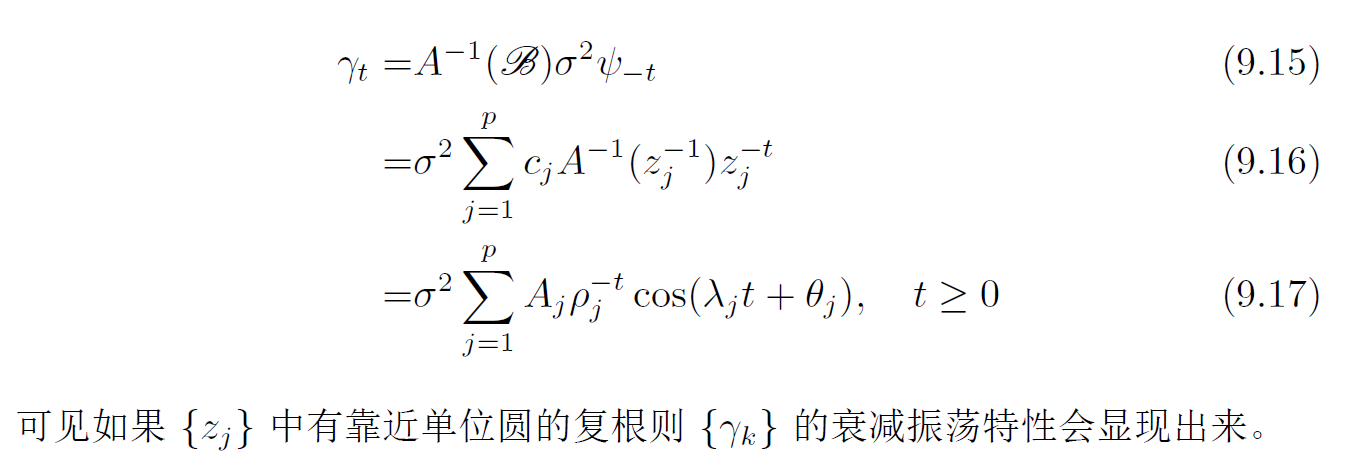
\includegraphics[width=0.70\textwidth]{5.png}  
	\end{figure}
$$T=\frac{2\pi}{\lambda_j}$$
\end{solution}

\item[6.]平稳序列经过线性变换后得到的序列还是平稳的吗?两个平稳序列的和序列还是平稳的吗?两个平稳序列的和序列的谱密度函数是对应序列的谱密度函数的和吗?
\begin{solution}
	1.平稳序列经过线性变换后得到的序列还是平稳的
	
	2.两个平稳序列的和序列:
	\begin{figure}[H]
		\centering
		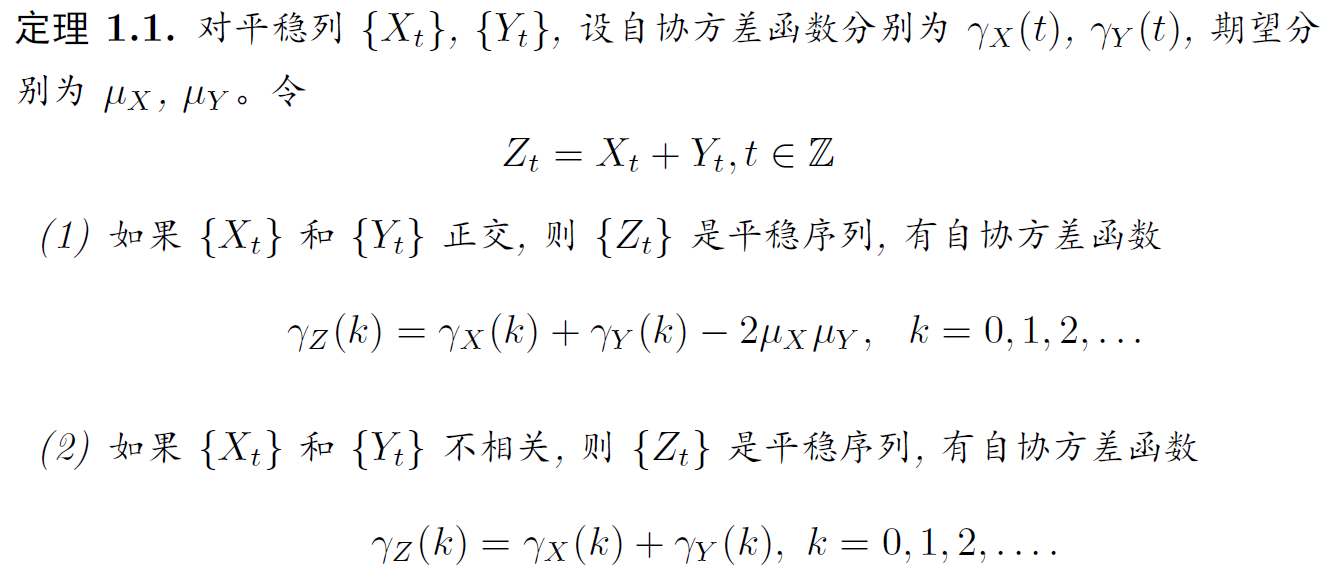
\includegraphics[width=0.75\textwidth]{1.png}  
	\end{figure}

3.两个平稳序列的和序列的谱密度函数当然不一定是对应序列的谱密度函数的和:
\begin{figure}[H]
	\centering
	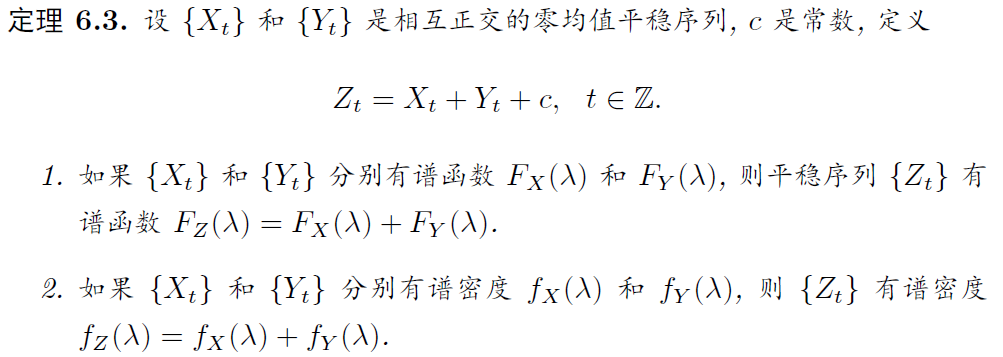
\includegraphics[width=0.75\textwidth]{6.png}  
\end{figure}
\end{solution}

%=================================================================%
\end{enumerate}
\end{document}